\documentclass[11pt,titlepage]{article}

\usepackage[margin=1in]{geometry} 
\usepackage{long table} % long tables
\usepackage{pdflscape}
\usepackage{graphicx}


\title{MOSES Flight Software \\ A Guide to the Source}
\author{David Keltgen, Roy Smart, Jackson Remington}
\date{\today}

\setlength{\textwidth}{14.5cm}

\begin{document}

\maketitle
\tableofcontents
\newpage

\section[Revisions]{Revision History}
	\begin{longtable}{|c|c|r|r|}
		\hline
		Revision	&	Date	&	\multicolumn{1}{c|}{History}	&	\multicolumn{1}{c|}{Initial}\\
		\hline
		0.1	&	03-11-2015	&	Created	& DJK	\\
		\hline
		0.2 & 4-26-2015 & Updated & RTS \\
		\hline

	\end{longtable}
	
\newpage


\section{Introduction}
\hrulefill
\\
The MOSES instrument is a sounding rocket payload designed to take exposures of the Sun in Extreme Ultraviolet wavelengths. Since the sounding rocket trajectory guarantees only 5 minutes of viable exposure time, the flight software must be able to operate nearly autonomously for the entire flight. Additionally, the flight software must also be able to be controlled from the ground to be able to integrate and test the instrument properly.\par

MOSES first launched in 2006 using flight software developed by Reginald Mead in C++, running on a Hercules EBX flight computer. Unfortunately this old flight computer started to develop electrical problems and could not be replaced. These events necessitated the selection of a new flight computer and development of new flight software. The new configuration was designed very similar to the original configuration in that an FPGA is utilized to capture the experimental data from the cameras, and that data is transferred back to the flight computer using Direct Memory Access. As a result the flight software is similar to the software developed by Reginald, except that it is written in C. \par

While the old flight software certainly performed as expected on the 2006 flight, the developers of the updated code made many attempts to fix or implement features that were not implemented in time for the first flight. These include: reducing the latencies between subsequent exposures, a well tested telemetry module, and good integration between ground station software and flight software. \par

With all that being said, the developer must note that this document is not intended as a Software User's Guide. It is designed to be a resource for the maintainer of the MOSES flight software and to provide a source code level description of the program. While all attempts will be made to make this document as accurate as possible, there will inevitably be errors that creep into this writing. The source code is the main source of information on the operation of the flight software, and an in-depth understanding of the software will only be possible through reading the source.

%\documentclass[11pt]{article}
%\begin{document}
\section{Main Subsystems}
\hrulefill
\\
Main Subsystems...
	\begin{enumerate}
		\item Tri-M VDX104+ : Main flight computer board. Contains the CPU, SD hard drive, RS-232 ports.
		\item CTI FreeForm PCI-104 Virtex 5 FPGA: Connected to the VDX104+ through PCI bus. Main function is to capture science data produced by the ROE. Also implemented on the FPGA is all of the output/input GPIO lines required for operation.
		\item Read-out Electronics (ROE):  The ROE is the interface between the FPGA and the CCDs that capture scientific data. Upon receiving a command from the flight computer to begin readout it will clock the data contained within the CCDS and stream it to the FPGA.
		\item Power board: Board that manages the power systems on the instrument. The flight computer applies a high value to whichever power subsystems have been requested to be activated and then strobes a latch to turn on/off the subsystems.
		\item Power board: Board that manages the power systems on the instrument. The flight computer applies a high value to whichever power subsystems have been requested to be activated and then strobes a latch to turn on/off the subsystems.
		\item Telemetry transmitter: Science data is sent from the FC to a radio transmitter, which sends the data back to the ground at 10 Mbit/sec
		\item Housekeeping link: Consists of two separate radio connections, hkup and hkdown. Hkup operates at 1200 baud and sends commands from the ground to the instrument. Hkdown operates at 9600 baud and sends replies from the instrument to the ground.
	\end{enumerate}

%\documentclass[11pt]{article}
%\begin{document}
\section{Requirements for Operating the MOSES Instrument}
\hrulefill
\\
\begin{enumerate}
  \item Operate power systems on the instrument. The power systems include: 
	\begin{enumerate}
		\item Shutter Driver: Must be activated to control the shutter.
		\item ROE: Must be activated to readout and flush the CCDs for exposures.
		\item Premod Filter: This system must be activated for high-speed telemetry to be used. It uses a hardware random number generator to randomize the telemetry data. This is important as the telemetry stream must have equal numbers of ones and zeros to be properly reconstructed on the ground. \textbf{NOTE: The Premod filter is a deprecated system and will no longer be used for MOSES-III and subsequent missions.}
		\item Temperature Control Systems: These systems provide cooling to the instrument while under vaccum. The CCDs are cooled using this system to minimize the noise inherent in the CCDs. The flight computer must also be cooled under vacuum to prevent overheating, as it is normally air-cooled. It must be noted that this system is NOT to be turned on while the instrument is at atmospheric pressure.
		\item 5V Regulator: This must be on to provide the premod filter with a -5V rail.
		\item 12V Regulator: Among other things, this subsytem activates the analog telemetry monitoring.
		\item H-$\alpha$ Camera: This camera is used in flight as a targeting system, to ensure the attitude of the payload is appropriate. This is an analog system, so the data produced by the H-$\alpha$ camera is not moderated by the flight computer, it is only activated through the flight computer. \textbf{NOTE: The H-$\alpha$ Camera is no longer being used for MOSES-III and subsequent missions. For the MOSES-III/ESIS mission, the ESIS instrument will be responsible for pointing the payload.}
	\end{enumerate}
The flight software is directed to turn on/off power systems through HLP packets sent by the EGSE.

  \item Control the read-out electronics (ROE). This is accomplished using an RS-422 serial connection between the FC and the ROE. Common task include: commanding exposures, flushing the CCDs, and requesting housekeeping data such as voltages and currents.
  
  \item Open and close the Shutter. The Shutter depends on two GPIO lines (open and close) and each must be pulsed for 200ms to execute their respective operations.

  \item Receive and save science data. Through the SPU, the ROE sends science data over a 32 Mbit/sec parallel connection. The FSW should have low enough latency so as to not miss any science data. The FSW should save each image as a 16 MB file with the extension .roe.
  
  \item Create an index of the images that were captured. This index is critical to the IDL software used to analyze MOSES images. This index should contain the name of the file, the number channels in the file

  \item Send science data over telemetry. NASA has provided a 10 Mbit/sec serial line that connects with a radio to the ground. During the course of the mission. While there is not enough time to send all of the data, the MFSW should send as much science data back to earth as possible to mitigate data loss from the harsh re-entry environment.

  \item Respond to Timers and Uplinks. Timers are single lines provided by NASA that instruct the instrument when to execute the different parts of the experiment. Timers include: 
	\begin{enumerate}
		\item Dark Exposure Start: These exposures don't open the shutter while taking an exposure. They are used to provide a baseline for the CCDs for data analysis post-flight.
		\item Data Start: This command carries out the data sequence outlined in a sequence file (to be explained later).
		\item Data Stop: Stops the current sequence whether it be a dark sequence or a data sequence. The sequence stops only after the current exposure has completed. Note: This command only stops the current data sequence. If there is more than one data sequence enqueued to the Science Timeline, the FSW will just start the next sequence following Data Stop.
		\item Sleep: Instructs the flight software to stop and to shut down the computer. This is important as we don't want the flight computer to be damaged during reentry into the atmosphere.
	\end{enumerate}
 Dark exposures are those which don't open the shutter while the CCDs are being exposed during the Science Timeline. Uplinks are similar to Timers in that they have the same functionality, except they are tied to a physical button on the ground. Using this interface, a user could control the experiment from just the push-button on the EGSE tower. 

  \item Respond to HLP packets. These packets are sent by the EGSE software on the ground, and provide all the functionality of Uplinks and Timers while providing additional commands to control the instrument. Two RS-232 connections are provided by NASA to facilitate this interface: HKUP and HKDOWN. Possible types of HLP packets include:
	\begin{enumerate}
		\item Uplink: Provides the same functionality as Uplinks initiated through the GPIO interface (e.g. Data Start, Data Stop, etc.)
		\item Shell: The FSW opens a bash shell as a child process. Shell packets can execute bash commands on the FC via this interface.
		\item Power: Queries, activates or deactivates power subsystems.
		\item Housekeeping Requests: Requests housekeeping data from the ROE.
		\item Mission Data Acquisition Requests: Allows direct control over exposure parameters and can also control the ROE.
	\end{enumerate}
The HLP interface is the main interface used for debugging and testing the instrument. This interface is also important during flight as it sends packets that inform the users of the current state of the FSW.
	
\end{enumerate}


%\documentclass[11pt]{article}
%\begin{document}
\section{Architecture Description}
\hrulefill
\\
The MOSES instrument needs to be able to respond to IO on several different interfaces. This is problematic in sequential programming, as input could be lost while the computer is in a another part of the program or output could be lost while the software is waiting for something else. This issue is alleviated by using a threaded software architecture, which can execute separate subprograms concurrently. Linux provides excellent libraries for threaded programming, known as POSIX threads (pthreads). Pthreads allows the flight software to execute the science timeline, while still being available to respond for input or write data to the hard-disk drive. 
The challenge with this threaded architecture is one of synchronization. Each thread operates independently, and steps must be taken to ensure that the program executes in the proper order and no memory is accessed simultaneously by two or more threads. In the MSFW thread synchronization is accomplished through so-called lockingQueues. lockingQueues are like a normal queue data structure, except that they take advantage of mutex locks to “lock” the queue until the accessing thread has completed its operation on the queue. LockingQueues are implemented anywhere in the program where it is necessary to pass data in between threads.
Another thread synchronization technique utilized in the MFSW is signals. Signals are objects provided by the Linux OS that allow separate threads or processes to get each others attention through a binary flag. In the MFSW, signals are used to instruct the main process to shut down the flight software.

\begin{landscape}
\begin{figure}[h!]
\centering
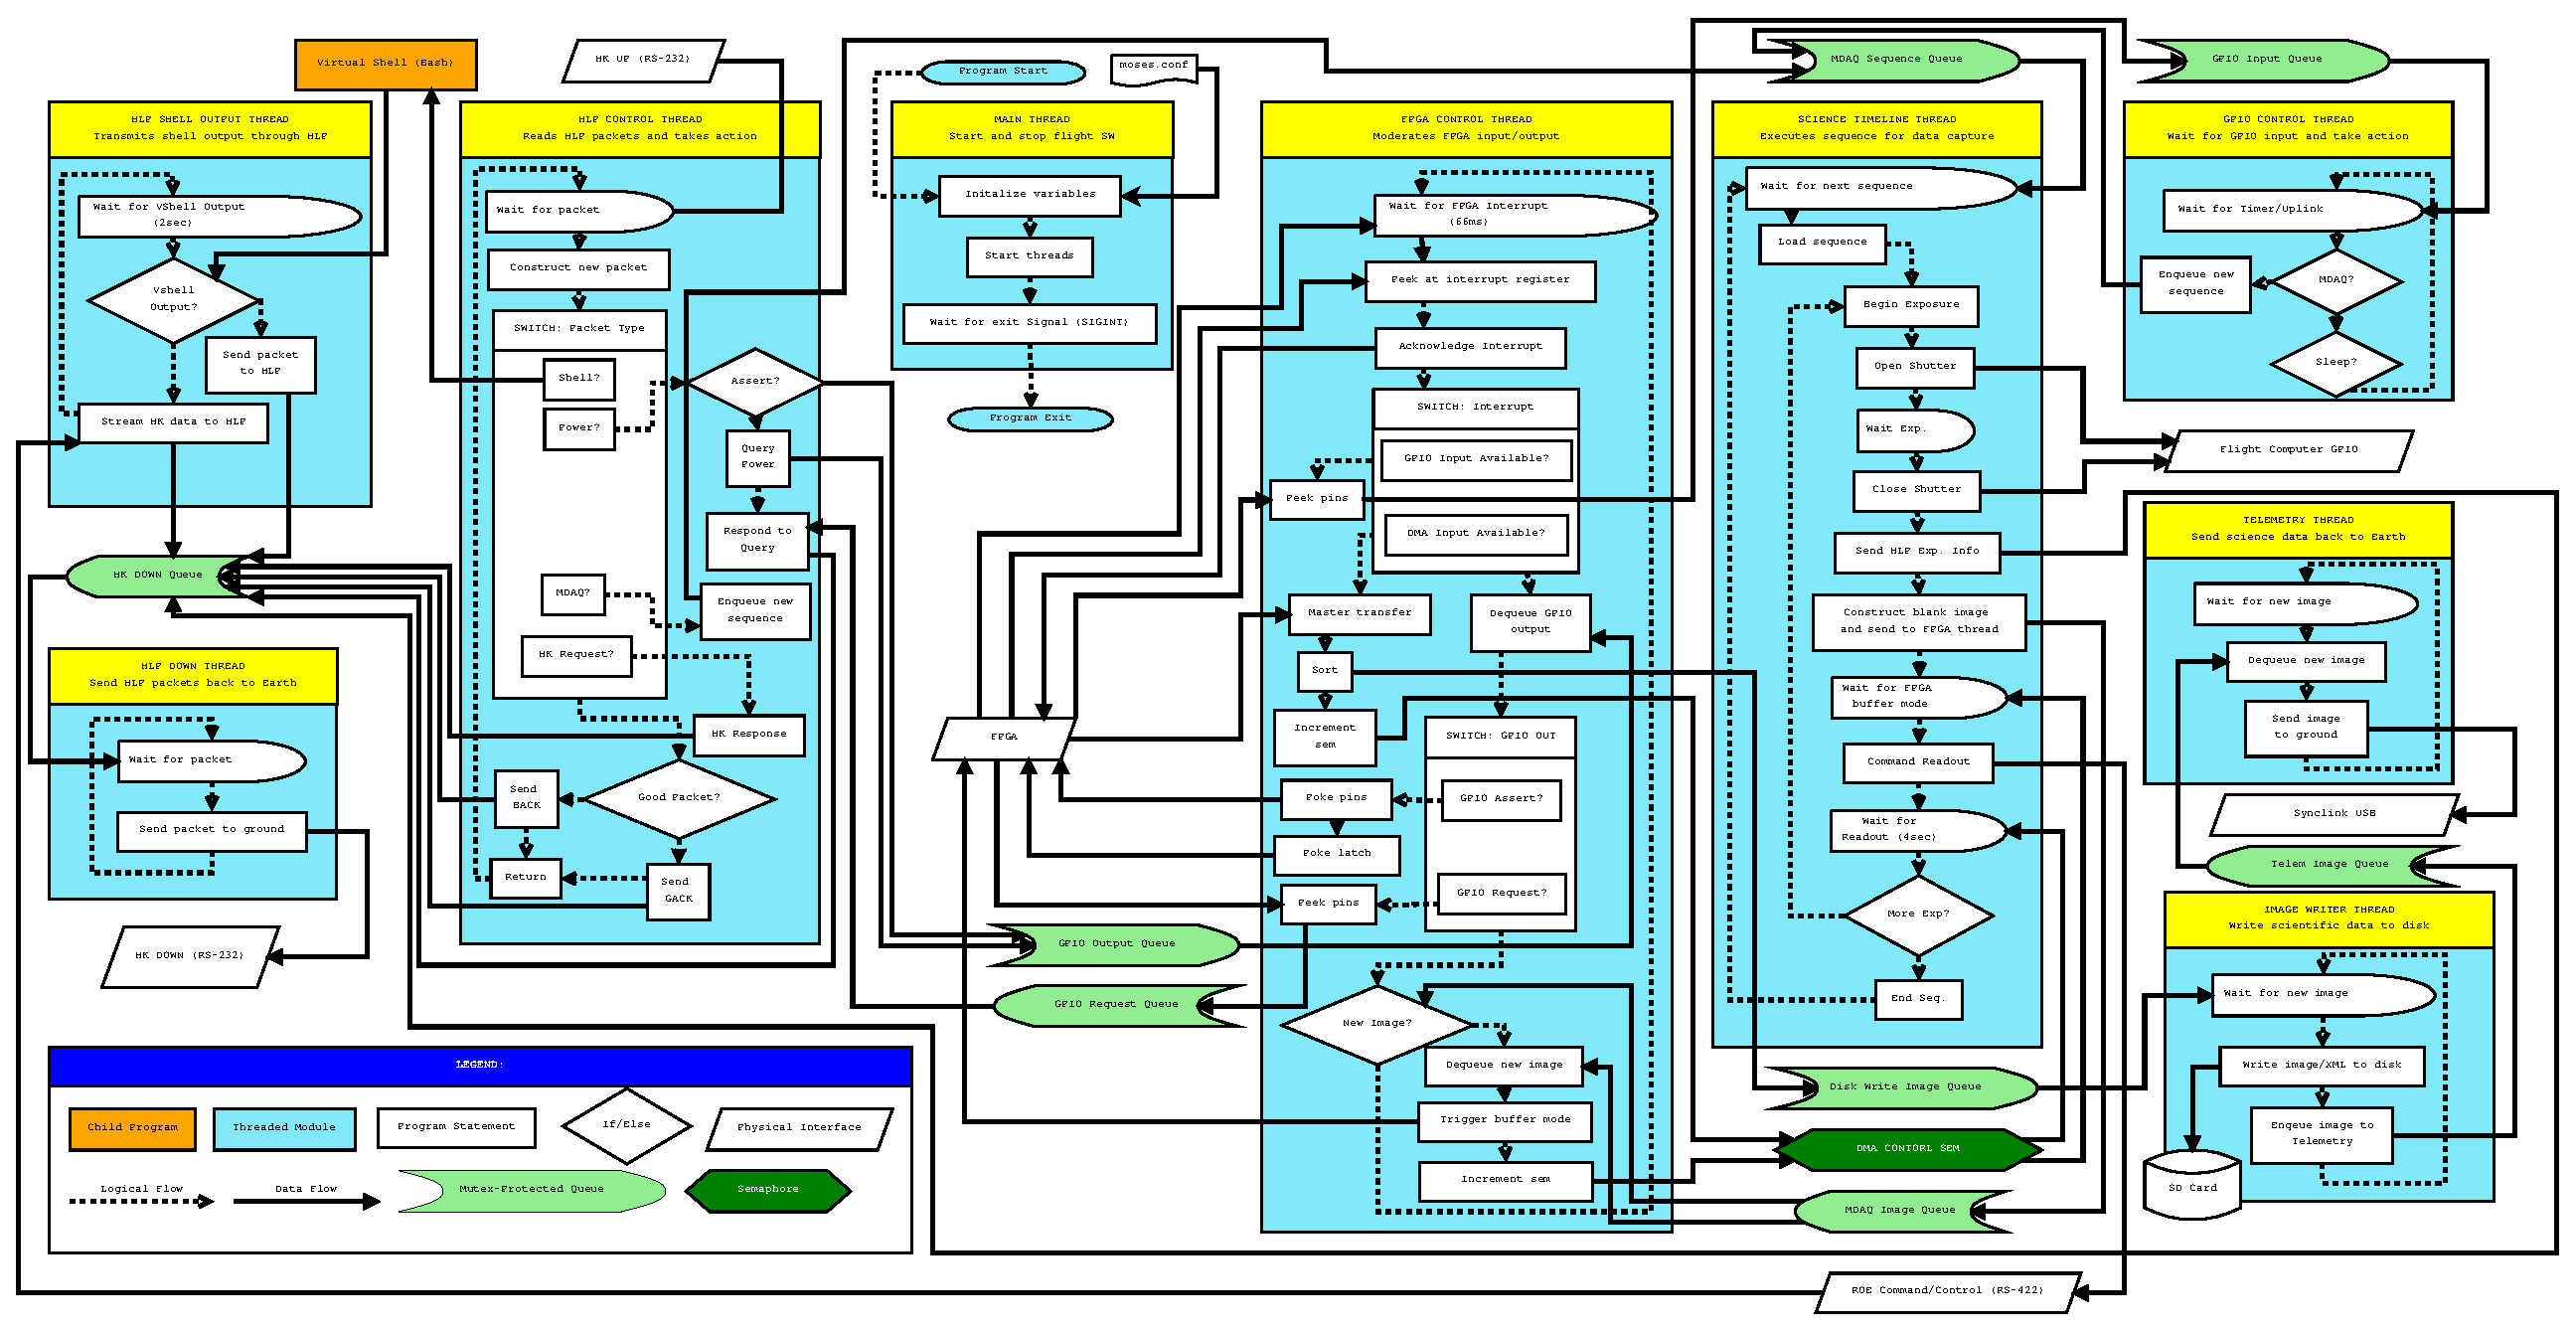
\includegraphics[width=24.5cm]{images/mfsw_block}
\caption{Block diagram summarizing the flight software architecture.}
\end{figure}
\end{landscape}
%\documentclass[11pt]{article}
%\begin{document}
\section{Main Thread}
\hrulefill
\\
Program initialization begins with the configuration file \texttt{moses.conf}. Each setting in the file specifies an individual thread or method of communication and is assigned a one (ON) or zero (OFF) for toggling during the debug process. After reading the configuration file, the Main thread starts the \texttt{bash} subprocess and notes its Program ID (PID). This will be used to kill the \texttt{bash} subprocess upon program exit. Then the Main thread proceeds to start each thread specified as active by \texttt{moses.conf}. The order of threads in \texttt{moses.conf} designates their load order; i.e. items listed higher will have higher execution priority. During flight, every option shall be set to ON. 

After each thread has successfully started, the Main thread is paused and simply waits for program exit. To exit the program any one of the threads may send a \texttt{SIGINT} Linux signal to the main thread to inform it of program shutdown. The main thread is waiting for this signal, and once it is raised, it will begin the process of cleaning up threads and exiting the program.
%\documentclass[11pt]{article}
%\begin{document}
\section{Science Timeline Thread}
\hrulefill
\\
Sci ti Thread...
As the name implies. the Science Timeline thread controls the overall experiment schedule. It starts off by ensuring that the ROE is active, otherwise the taking exposures would be pointless. Like all of the threads, Science Timeline is initialized at startup, but waits on a signal ('SIGUSR1') in order to continue. Once it has been received, the thread will set the current sequence from the already-initialized sequence map and begin taking exposures. The 'takeExposure' function starts off by flushing the ROE Charge-Coupled Devices (CCDs) 5 times in order to remove any accumulated charge. It then opens the shutter and then uses a sleep function to wait for the designated exposure time (timing experiments to determine accurate sleep times are still to be done). If the exposure is a data sequence, then additional time will be added to the exposure length as represented by the variable PULSE in 'sciencetimeline.h.' This additional time is used to account for the difference in the time it takes to open and close the shutter. 
Once the exposure is taken, meta data of the image is saved to the data structure. After that, the thread commands the ROE to read out its exposure data. This process will take four seconds, and this thread can sleep during that time (to free other processes). Science Timeline's last task to complete is to enqueue the image to the image-writing thread to independently start writing data to the SD card while the science timeline thread moves to the next exposure. 
This process is repeated for each exposure in the specified sequence.

\subsection{Read Out Electronics (ROE)}

The ROE is capable of being in several different modes. Those different modes are:

\textbf{Default Mode:}
This is the mode that the ROE is initially in on startup. In default mode, only one command can be sent to it, which is the exitDefault() command. While in default mode, all the ROE does is simply readout an exposure every twelve seconds.

\textbf{Command Mode:}
This is the mode that the ROE is in after the exitDefault() command has been sent. The ROE will be in command mode for the majority of the flight. In this mode, commands can be sent such as setting the ROE to a new mode, reading out the CCDs or requesting Housekeeping values. 

\textbf{Selftest Mode:}
In selftest mode, the ROE will not read out the CCD’s at all, but will instead read out a predefined sequenceof vertical bars. This can be useful for testing the flight computers data acquisition abilities. Once the ROE is in selftest mode, it must be reset via the reset() method in order to exit selftest mode. One would also need to exit default mode again after the reset.

\textbf{Stims Mode:}
In stims mode,  a predefined pattern is generated in much the same way as the selftest pattern. The difference is that in stims mode the pattern is fed through the CCD readout circuits and thus any extraneous noise and other anomalies show up in the pattern. Also, unlike selftest mode, stims mode can be exited by using the stimOff() method.

\textbf{Nominal Operation}

The ReadOutElectronics object is instructed to exit default mode, reset, and then exit default mode again. The cause for this seeming redundancy is that commanding the ROE to exit default mode while in command mode has no effect. However, commanding the ROE to reset while it is in default mode causes a software error. Therefore, we exit default mode once to make sure that the ROE is commandable, tell it to reset so that we know what configuration it is in, and then finally exit default mode again to make it commandable in a known configuration. The default port for the ROE is /dev/ttyS1 (COM2).
The main job of the ROE is to read out the data on the CCD cameras. The two main functions required to acheive this are the flush() and readout() functions. Flush is used to clear any accumulated data on the cameras and readOut is used to get the data from the cameras. The biggest difference between the two, is that flushing the ROE is faster and doesn’t send any data down the data link. It is recommended that the ROE be flushed five times in succession before every exposure. Readout does just what one would expect, it reads out the cameras. It is suggested that the ROE be allowed four seconds for reading out data between exposures. The only notable point of confusion for this method is that it also requires a block id, which is basically just a byte that defines how the ROE needs to be read out. There are unique id’s for reading out the ROE normally, reading out while in selftest mode, reading out while in stims mode, and there are even some undocumented id’s which were used for testing during the construction of the ROE. All of these block id’s are documented in the roe.h file.

As a last point of interest, there are also methods for getting and setting the analogue electronics parameters inside the ROE. These methods normally go unused and
are usually only useful during testing. These parameters consist of 8 bytes which control
the ROE’s behavior. In fact, it is by setting these values that the ROE is placed into
selftest and stims mode. In those methods these parameters are written automatically.
It is suggested that these parameters only be changed if an experienced ROE operator
/technician knows what they are doing.


In regards to the Housekeeping data of the ROE, the values that are returned are the raw hex values. These raw hex values are then passed on from the flight software to the ground station. The ground station then displays these raw values, unconverted.

Mutex locks have been implemented in the ROE functions since multiple threads could potentially be trying to access it at the same time. An example of this could be that the Science timeline thread could be telling the ROE to flush the CCD’s, while a packet sent from the GSE could be requesting HK values. Although the likelihood of this clashing of threads causing errors in small, it is important to make sure that the signals being sent to the ROE are exactly what we intended them to be.





%\documentclass[11pt]{article}
%\begin{document}
\section{Image Writer Thread}
\hrulefill
\\

Through time testing, it was determined that previous revisions took approximately one second to write each ROE image to disc. Since this mission is very time-critical, such a delay was deemed too long to fit serially in the Science Timeline thread. Moving it to another results in a large percentage of flight time saved, allowing more exposures to be captured per flight.
A ROE image structure is used to store all the image data and meta data for each successful image. Here is a brief overview therein:

Identifying values for the origin, instrument, observer, and object will typically not change on each flight. However, if this software were to be used under different circumstances, these values could be changed to reflect that. 'Bitpix,' the bits per pixel value, along with the images' width and height, are set...(???) 'Channels' consists of a single character value that can be ANDed and ORed with defined values to enable or disable each channel as required. For ideal exposures, channels 1, 2, and 3 will be enabled while channel 0 (noise) is disabled. Other values unique to each image include the filename, its path, the date and time its exposure started, its duration, the size in pixels of each channel, as well as the total number of exposures in its sequence.  

The image writer thread starts by assigning data to the image structure inside the 'write\_data' function. Once all of these values are assigned, it goes to write the file. This is subsequently broken down into two tasks: writing the actual image data to disk, and writing the record file (imageindex.xml) to disc. The xml file contains all of the metadata. 

Rather than be discarded after saving, the files are kept in memory (aside from the noise channel, which is only saved locally). A pointer to it is placed into the telemetry queue for transmission to the ground. This way, many images may be retrieved before touchdown and without requiring survival of the payload. An updated version of the xml file is also sent to the queue between each image.


%\documentclass[11pt]{article}
%\begin{document}
\section{GPIO Control Thread }
\hrulefill
\\
GPIO Thread...

%\documentclass[11pt]{article}
%\begin{document}
\section{FPGA Server}
\hrulefill
\\
The FPGA Server thread mediates communications with the FPGA and the rest of the flight software. The FPGA is critically important to the goals of the MOSES instrument, as it is the electronics that receives the experimental data from the cameras, as well as managing the GPIO input/output lines which control the instrument and the execution of the flight software. Since there are many different threads that depend on the FPGA for their execution, we implemented the FPGA Server thread to avoid thread contention issues between different parts of the program.

%\documentclass[11pt]{article}
%\begin{document}
\section{Housekeeping Link Protocol (HLP)}
\hrulefill
\subsection{HLP Control Thread}
The HLP Control thread listens for incoming HLP packets and then takes the appropriate action based on the content of the packet.

\subsection{HLP Down Thread}
The HLP Down thread is attached to the HLP Down queue. As the different threads in the flight software produce HLP packets that need to be sent to ground, they enqueue it onto the HLP Down queue. The HLP Down thread dequeues these packets one-by-one and sends it to the ground via a RS-232 serial port.

\subsection{Virtual Shell}
The Virtual Shell is an alternative way to write commands to the flight computer, rather than performing an \texttt{ssh} into the flight computer. Commands typed into the virtual shell are wrapped in HLP packets and are sent to the flight computer, where it is then executed.

\subsection{HLP Shell Output Thread}
The HLP Shell Output thread waits for output from the virtual shell, and if there is an output, it is sent to the HK Down queue. From there it is sent to the HLP Down thread. See Figure 2 for a more detailed description of threads in the flight computer.

\section{High-Speed Telemetry}
\hrulefill
%\documentclass[11pt]{article}
%\begin{document}
\section{\bf Dictionary of Abbreviations }
\hrulefill
\\
\begin{enumerate}

\item HLP - Housekeeping link protocol
\item ROE - Read-out electronics
\item FC - Flight computer stack (VDX + FPGA)
\item MFSW - MOSES flight software
\item VDX - VDX104+ (Flight computer)
\item GSE - Ground station equipment

\end{enumerate}



\end{document}
